\documentclass{sigchi}

% Use this command to override the default ACM copyright statement (e.g. for preprints). 
% Consult the conference website for the camera-ready copyright statement.
\toappear{
  Submitted for review.
}

% Arabic page numbers for submission. 
% Remove this line to eliminate page numbers for the camera ready copy
\pagenumbering{arabic}


% Load basic packages
\usepackage{balance}  % to better equalize the last page
\usepackage{graphicx} % for EPS, load graphicx instead
\usepackage{times}    % comment if you want LaTeX's default font
\usepackage{url}      % llt: nicely formatted URLs
\usepackage{subfigure}
\usepackage{tikz}

%\linespread{2}

% llt: Define a global style for URLs, rather that the default one
\makeatletter
\def\url@leostyle{%
  \@ifundefined{selectfont}{\def\UrlFont{\sf}}{\def\UrlFont{\small\bf\ttfamily}}}
\makeatother
\urlstyle{leo}


% To make various LaTeX processors do the right thing with page size.
\def\pprw{8.5in}
\def\pprh{11in}
\special{papersize=\pprw,\pprh}
\setlength{\paperwidth}{\pprw}
\setlength{\paperheight}{\pprh}
\setlength{\pdfpagewidth}{\pprw}
\setlength{\pdfpageheight}{\pprh}

% Make sure hyperref comes last of your loaded packages, 
% to give it a fighting chance of not being over-written, 
% since its job is to redefine many LaTeX commands.
\usepackage[pdftex]{hyperref}
\hypersetup{
pdftitle={SIGCHI Conference Proceedings Format},
pdfauthor={LaTeX},
pdfkeywords={SIGCHI, proceedings, archival format},
bookmarksnumbered,
pdfstartview={FitH},
colorlinks,
citecolor=black,
filecolor=black,
linkcolor=black,
urlcolor=black,
breaklinks=true,
}

% create a shortcut to typeset table headings
\newcommand\tabhead[1]{\small\textbf{#1}}


% End of preamble. Here it comes the document.
\begin{document}

\title{Gesture Beyond the Surface: Online Continuous Gesture Recognition}

\numberofauthors{2}
\author{
  \alignauthor 1st Author Name\\
    \affaddr{Affiliation}\\
    \affaddr{Address}\\
    \email{e-mail address}\\
  \alignauthor 2nd Author Name\\
    \affaddr{Affiliation}\\
    \affaddr{Address}\\
    \email{e-mail address}\\
}

\maketitle

\begin{abstract}
Non-touch gestures are useful for interacting with large displays. We have developed 
a gesture salience detection method for gesture recognition. 
It shows a better result than both dense sampling and using 
Kinect skeleton tracking. We also developed an online
continuous gesture recognition framework based on an abstract hidden Markov model
which  handles both unbounded and
unsegmented input. Our evaluation shows that a small time lag (about 0.5s) in online inference 
can give comparable results with offline
smoothing. We also show that AHMM based recognition gives better results than the mixture of HMMs method because it learns transition probabilities across gestures.

\end{abstract}

\keywords{
Gesture recognition; abstraction hidden Markov models; feature detection; histograms of 
oriented gradients.
}

\category{H.5.2.}{Information Interfaces and Presentation (e.g. HCI)}{User Interfaces}

\section{Introduction}
The introduction of inexpensive RGB-D(epth) cameras such as the Kinect sensor from Microsoft or the Carmine from Primesense
has made markless motion capture relatively easy. Their increased popularity indicates people's desire for more
natural and less restricted interaction with computers. Especially with large tabletop
and wall displays, the ability to interact with the interface at a distance without touching can provide great
convenience for users.  

We have developed an online continuous gesture recognition framework to enable gesture interaction beyond the surface
of large displays, using a RGB-D camera. The framework works for both horizontal tabletop displays and vertical displays.
For a horizontal tabletop, the camera is placed directly above, looking down at the interface; for a vertical display, 
the camera is placed near the display, looking towards the user. 

An abstract hidden Markov model (AHMM) based gesture recognition framework
will work for both kinds of displays. Our earlier work (under submission) applied it to gesture recognition in the tabletop environment.
In this paper, our focus is on vertical display.
The only difference is the feature extraction method. Hand tracking for the tabletop display may be easier because the 
background is just the display, which is usually flat and static. For a vertical display, hand tracking can be more challenging, as the view 
from the camera is more complicated.

In this paper, we describe our method of gesture salience detection for vertical display interaction. We also describe the AHMM-based
gesture recognition framework, which can handle unbounded and unsegmented input features for online continuous gesture recognition.

Using a public gesture corpus for evaluation, we show that our gesture salience detection gives a better recognition result than both dense sampling and using 
Kinect skeleton tracking. We also show that a small time lag (~0.5s) in online inference using our recognition framework can give comparable results with offline
smoothing. Furthermore, our evaluation indicates that AHMM based recognition gives better results than the mixture of HMMs method because it learns transition probabilities across gestures.

\section{Related Work}
Our work can usefully be compared with other work with respect to: gesture feature detection and gesture/action classification.  

\subsection{Feature Detection}
Common feature detection for gesture recognition involves hand tracking based on skin detection~\cite{shin2004} or motion detection~\cite{cutler1998}.
Skin detection in an HSV~\cite{Bradski98} or YCrCb color space can be relatively robust and less sensitive to lighting conditions,
compared to a RGB color space. However there still can be other materials 
with skin-like colors (such as clothes) that can produce false positives. Skin from other parts of the body can also interfere with hand tracking. 
Shin et at.~\cite{shin2004} filter out false positives by considering the skin blob closest to the camera. However this can fail when the hand is close to
the body, generally resulting in the face being detected instead. Methods based on motion-only detection would assume the background is relatively static and there is no motion at
the other parts of the body. In response, we consider skin, motion and closeness together to compute a probability map for gesture salience. 

Marcos-Ramiro et al.~\cite{marcos2013} developed a method of computing hand likelihood maps based on RGB videos
for extracting body communicative cues. They mention that, given a frontal, static camera pointing to the gesturer,  his/her hands are usually the closest
part to the camera, and also move with the highest speed. These characteristics translate to more movement in the image where
the gesturing hand(s) is. As they only use non-stereo RBG images, they can not actually compute the closeness of the movement, and compute the amount
 of motion using optical flow.
Our method is very similar to theirs, but we combine both RGB images and depth images to compute
the gesture salience. We also use depth data to compute the amount of motion which can be computationally less intensive than the optical flow method.

Laptev~\cite{laptev2003} introduced the space-time interest points (STIPs) and used them for human
action recognition from movies~\cite{laptev2008}. STIPs are points in the video sequence where the image values have
significant local variations in both space and time. His method is an extension of the Harris interest point detector from the spatial domain~\cite{Harris88}
to the spatial-time domain. For each cuboid of interest point, both histograms of oriented gradients (HOG)
and optic flow (HOF) are computed as feature descriptors. However, Wang et al.~\cite{wang-spatio-2009} compare several space-time feature detectors and
descriptors, including STIP, under a common experiment setup for human action recognition and find that dense sampling consistently
outperforms all tested interest point detectors in realistic video settings. They suggest this indicates the limitations of 
current interest point detectors.

Dense sampling is basically computing feature descriptors at regular positions and scales in space and time~\cite{wang-spatio-2009}.
It produces a very large number of features, which is more difficult to handle than the relatively sparse number of interest points.
Kone\v{c}n\'{y} and Hagara also used dense sampling and HOG and HOF features for gesture recognition. In our work, we compare our gesture salience detection and 
dense sampling method using the same gesture data set and recognition method. 

Another approach to hand tracking is based on 3D body pose estimation and searching for the hand region near the wrist~\cite{SongDD2011b}.
Skeleton tracking provided by the Kinect Software Development Kit (SDK) gives a relatively robust 3D body pose estimation. The tracking
is based on a body part detector trained from a random forest of a huge number of synthetically-generated poses~\cite{Shotton:2011}. One of its
major strengths is that it does not require an initialization pose. However, we observe that while the tracking for the head and shoulders are quite 
robust most of the time, the hand joint tracking fails when the hands are close to the body or are moving fast. In our experimental evaluation, we
 compare our method with a hand detection method based on the Kinect skeleton tracking.

\subsection{Gesture and Action Classification}
Hidden Markov models (HMMs) are commonly used
to model gestures with paths~\cite{sharma00, Starner95}. 
One HMM model is trained for each gesture class, resulting in a mixture of HMMs~\cite{yin10}. During
recognition, a segmented gesture sequence is presented to each HMM and the one that gives the highest
likelihood of the observed sequence determines the gesture class. Hence this method requires
a separate accurate gesture segmentation mechanism, which can be difficult to create, especially for online, continuous gestures
recognition.

Some researchers have used discriminative models (e.g., hidden conditional 
random fields (HCRF)~\cite{wang06}, or latent-dynamic conditional random fields (LDCRFs)~\cite{morency07}), which can provide some 
performance improvement over an HMM. But HCRFs
can handle only segmented gesture sequences and LDCRFs can handle only bounded sequences. Song et al.~\cite{song12} extend the LDCRF by 
adding exponential smoothing to the prediction at each time frame, but their model does not
use the end state of each gesture as a constraint to the gesture transition, and thus, may not
model the gesture production process adequately.  

Fran\c coise applied a 2-level hierarchical hidden Markov model (HHMM) for real-time 
gesture segmentation and recognition~\cite{francoise10}, but used a limited gesture set and basic features (e.g., accelerometer readings).
AHMMs and HHMMs are closely related, and both of them have been used to model user activities~\cite{nguyen03, nguyen05}. Our
previous work (under submission) compared these two models based on our gesture data set and showed that AHMMs gave a more accurate result.

Also for human action recognition, Laptev et al.~\cite{laptev2008} used a support vector machine (SVM) based classifier
on a bag-of-features computed from STIPs. The bag-of-feature (BoF) approach is similar to the bag-of-word approach in document classification.
To represent an image using the BoF model, an image can be treated as a document. 
``Words'' in images are identified through feature detection, feature description and code book generation~\cite{fei2005}.
An SVM does not usually handle time series data. To use an SVM on time series data, one
can concatenate the features in a time series into one long vector. However as the vector dimension (and hence the time window) needs to be fixed, it is not clear how this method can handle
gestures with different time length and speed.

\section{System Overview}
Our online continuous gesture recognition framework uses RGB and depth streams from a RGB-D (such as the Kinect) camera. Our goal is to enable
non-touch gesture interaction
with large tabletop displays and vertical displays. Two important parts to a gesture recognition
system include feature extraction and feature classification.  

\begin{figure*}
\centering
\includegraphics[width=1\linewidth]{figure/system.ps}
\caption{System overview of our gesture recognition framework. }
\label{fig:system}
\end{figure*}

Feature extraction on video sequences is often done in two steps: 1)
detect points of interest by maximizing certain salience functions; 2) compute
feature descriptors to capture shape and motion in the neighborhoods of the selected
points~\cite{wang-spatio-2009}.

For hand gesture recognition, the points of interest are certainly the hands. While the skeleton tracking provided
by the Kinect SDK is quite robust most of the time, its error for hand joint tracking increases when
the hands are close to the body or move quickly (see Figure~\ref{fig:compare-skeleton}). As a result, we
developed a gesture salience detection method to locate the gesturing hand more accurately.

After identifying the gesture salience region, we compute HOG feature descriptor 
on the image patch at the salience region. The final stream of feature vectors are input to the AHMM-based
gesture recognition framework for classification. Figure~\ref{fig:system} shows the overview of the entire process.
The following sections give detailed explanation of our method.  
 
\section{Gesture Salience Detection}

Similar to Marcos-Ramiro et al.~\cite{marcos2013}, we define gesture salience as a function of 
the closeness of the motion to the observer (e.g., the camera) and the magnitude of the motion,
and compute it from both the RGB and the depth data. Both the RGB and the depth data can be noisy. RGB cameras are sensitive to lighting conditions.
Skin color based detection can be sensitive to the clothes users wear. Depth cameras based on 
structured light sensors, such as the first generation Kinect sensor, compare the projected infra-red pattern
with the reflected one to determine depth~\cite{welsh:2011}. As a result, they do not work well on 
objects that are highly reflective (mirrors and shiny metal) or highly absorptive (fluffy and/or dark materials such as human hair)
\footnote{\url{http://msdn.microsoft.com/en-us/library/hh855356.aspx}}. By combining both RGB and
depth information
the overall gesture salience detection can be more robust.

The following are the detailed steps of our gesture salience detection method for each frame. 
We show the illustrations in Figure~\ref{fig:gesture-salience}. 

\subsection{Skin Segmentation}
To make our method generalizable to any users and environment, we use an off-the-shelf simple skin color detection method which is not trained on our data set to do a binary segmentation. 
. We compute a binary skin mask, $M^S$, based on the RGB image converted into YCrCb
color space.  We also find the user mask, $M^U$ obtained from the Kinect SDK based on the depth image. 
We then align $M^S$ with $M^U$ and find their intersection $M^{S\wedge U}$, which indicates the skin region on the user.

\subsection{Motion Detection}
Similar to Cutler and Turk~\cite{cutler1998}, we compute the motion mask for the current depth frame based on 3 frames. We first filter each 
depth frame by the user and skin mask $M^{S\wedge U}$ at time $t$, and then
smooth it through a median filter to obtain $D_t$, which is basically a depth image containing user's skin region only (see Figure~\ref{fig:skin-mask}).
Equation~(\ref{eq:motion-mask}) computes the binary mask, $M_{t\vee t-1}^M$, indicating pixels whose depth values have changed from time $t-1$ to $t$ (Figure~\ref{fig:motion-mask}).
$D_{t\vee t-1}^{D}$ is the absolute difference between $D_t$ and $D_{t-1}$, and $T$ is the threshold operator that filters out small change in depth value 
(we set the threshold to be 15mm). 
To obtain the motion mask, $M_{t}^M$ for time $t$ only, we use $M_{t-1\vee t-2}^M$, the motion mask for $t-1$ and $t-2$ as well (see Equation~(\ref{eq:motion-mask-t-1})-(\ref{eq:motion-mask-t}),
 AND and XOR indicated by $\wedge$ and $\oplus$).
\begin{align}
M_{t\vee t-1}^M &= T(D_{t\vee t-1}^{D}) \label{eq:motion-mask} \\
M_{t-1}^M &= M_{t\vee t-1}^M \wedge M_{t-1\vee t-2}^M \label{eq:motion-mask-t-1}\\
M_{t}^M &= M_{t\vee t-1}^M \oplus M_{t-1}^M \label{eq:motion-mask-t}
\end{align}

\subsection{Salience Map}
We compute histograms of depth values in both $D_t$ and $D_{t\vee t-1}^{D}$ and then apply histogram normalization to obtain cumulative distributions $H_t$ and $H_{t\vee t-1}^D$.
$H_t$ represents the probability of salience given a depth value, while $H_{t\vee t-1}^D$ represents the probability of salience given
a depth difference value. The lower the depth value or the higher the depth difference value, the higher the salience probability. The reason for using
histogram equalization is to reduce the effect of outliers such that a single large depth value will not suppress the salience probabilities of other depth values. 
Finally the salience map (Figure~\ref{fig:salience}) can be computed for each pixel $(x, y)$ as
\begin{align}
S_t(x, y) = H_t(D_t(x, y)) \times H_{t\vee t-1}^D(D_t^D(x, y)) \times M_t^M
\end{align}
The multiplication of the binary motion mask $M_t^M$ allows us to consider only the motion due to the user at $t$.
 
\subsection{Salience Location}
The final step of locating the most salient region in a frame is finding the
contour, $C_t$, from the salience map $S_t$ that has a perimeter greater than
the smallest possible hand perimeter and with the highest average salience for all the pixels inside the contour.

When motion is slow, the motion mask usually indicates the edge of the moving
object. As a result, the center of $C_t$ may not be the center of the moving
object (in our case, the user's hand). Hence, we use 2 iterations of Camshift~\cite{Bradski98} on the depth image $D_t$ with a start search location at the center of $C_t$ to refine
the final bounding box, $B_t$, of gesture salience (Figure~\ref{fig:camshift}).

\begin{figure*}[tb]
\centering
\hspace{-0.6em}%
\subfigure[]{
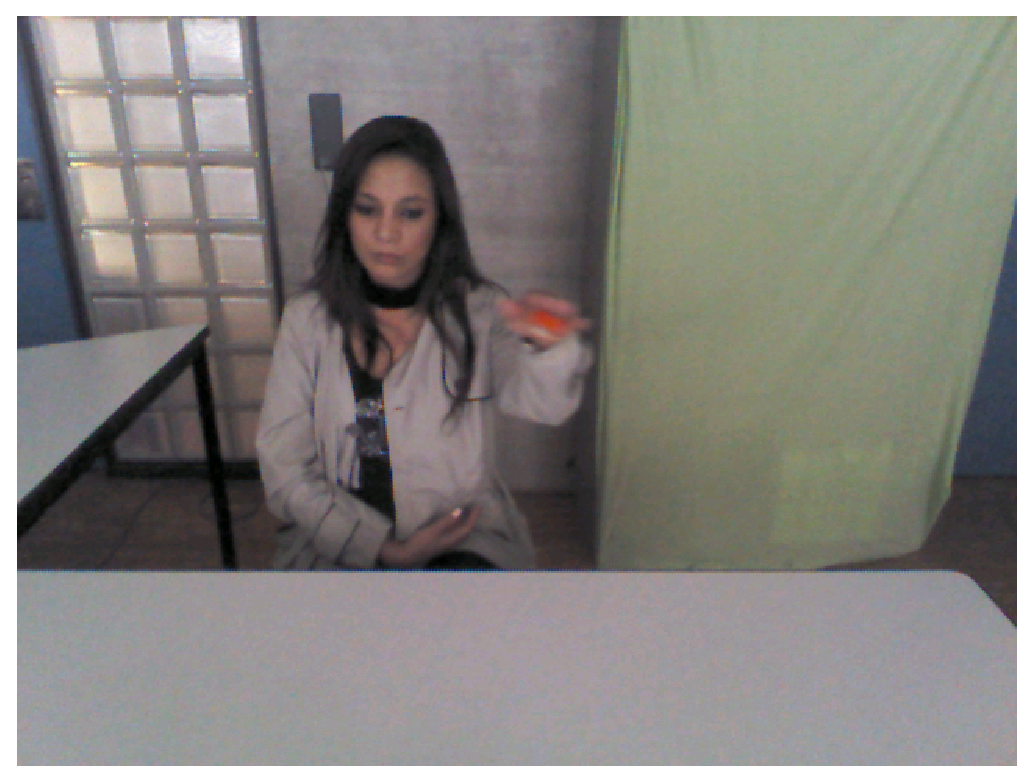
\includegraphics[width=0.195\linewidth]{figure/color.eps}\hspace{-0.6em}%
\label{fig:color}
}
\subfigure[]{
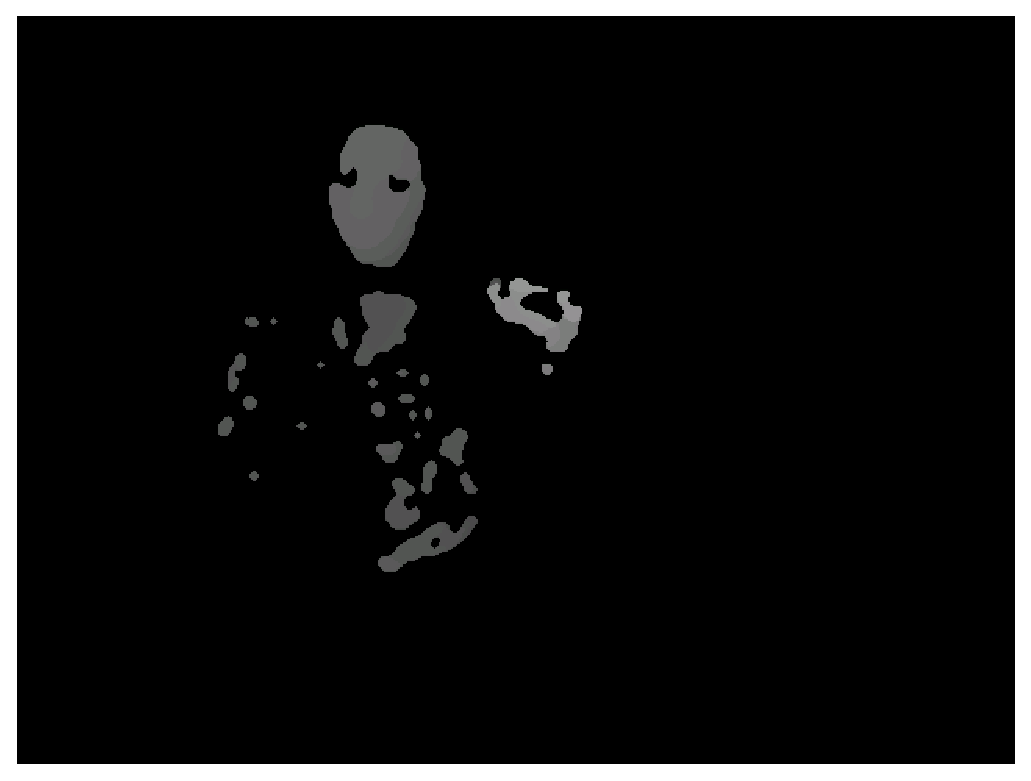
\includegraphics[width=0.195\linewidth]{figure/depth.eps}\hspace{-0.6em}
\label{fig:skin-mask}
}
\subfigure[]{
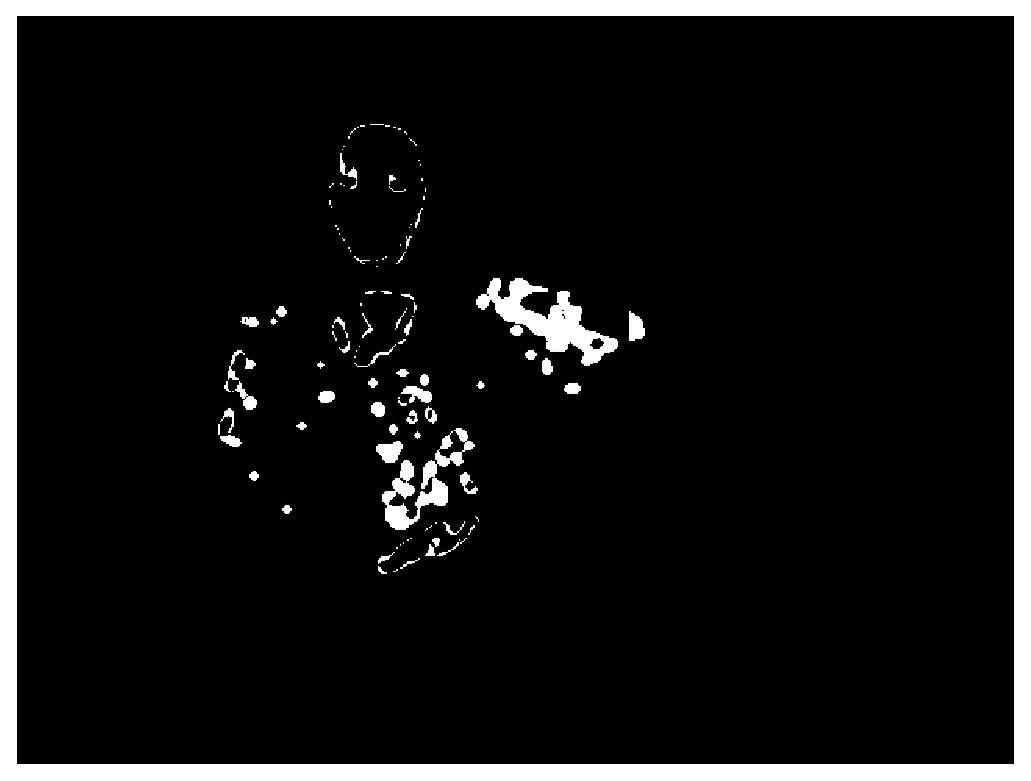
\includegraphics[width=0.195\linewidth]{figure/motion-mask1.eps}\hspace{-0.6em}
\label{fig:motion-mask}
}
\subfigure[]{
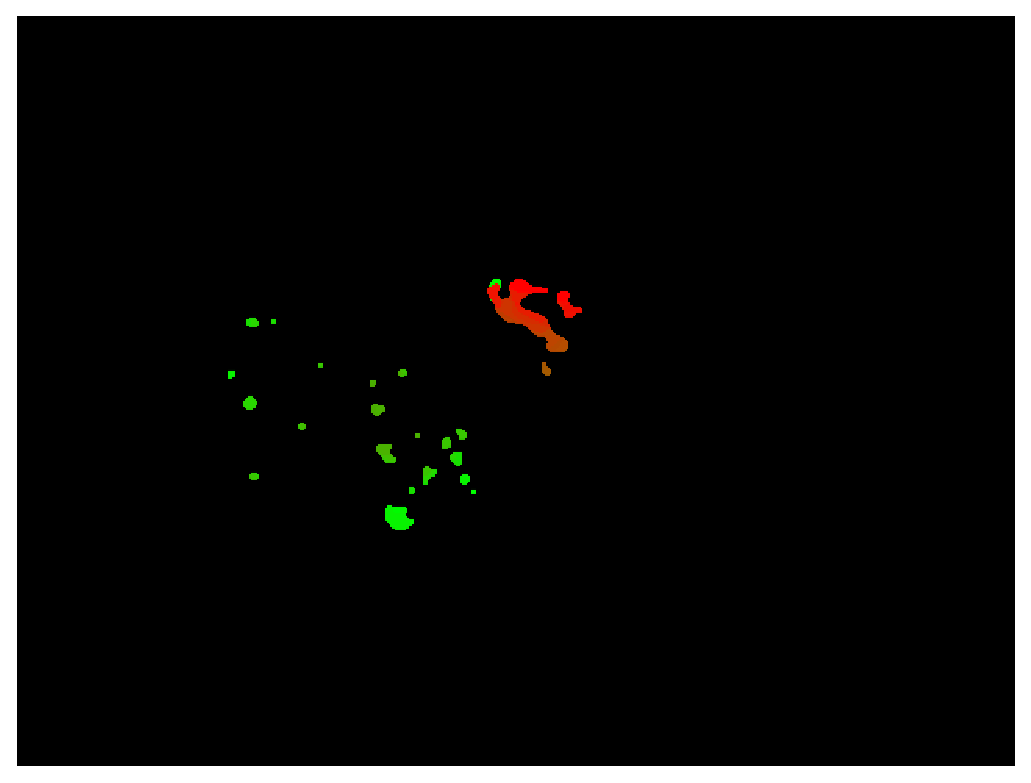
\includegraphics[width=0.195\linewidth]{figure/salient-map.eps}\hspace{-0.6em}
\label{fig:salience}
}
\subfigure[]{

\includegraphics[width=0.198\linewidth]{figure/bounding-box.eps}
\label{fig:camshift}
}
\caption{Gesture salience detection steps: \subref{fig:color} RGB image under low lighting condition;
\subref{fig:skin-mask} depth map $D_t$ filtered by skin and user mask, $M^{S\wedge U}$. False detection of skin due to
clothes color similar to skin color; \subref{fig:motion-mask} motion mask,  $M_{t\vee t-1}^M$, indicating moved pixels for time $t$ and $t-1$;
\subref{fig:salience} salience map with red color indicating high probability of the salience; 
\subref{fig:camshift} final gesture salience bounding box, $B$. (Best viewed in
color.)}
\label{fig:gesture-salience}
\end{figure*}

Figure~\ref{fig:compare-skeleton} compares the results of gesture salience detection for hand gestures with the skeleton tracking results
from the Kinect SDK.
\begin{figure*}
\centering
\subfigure[]{
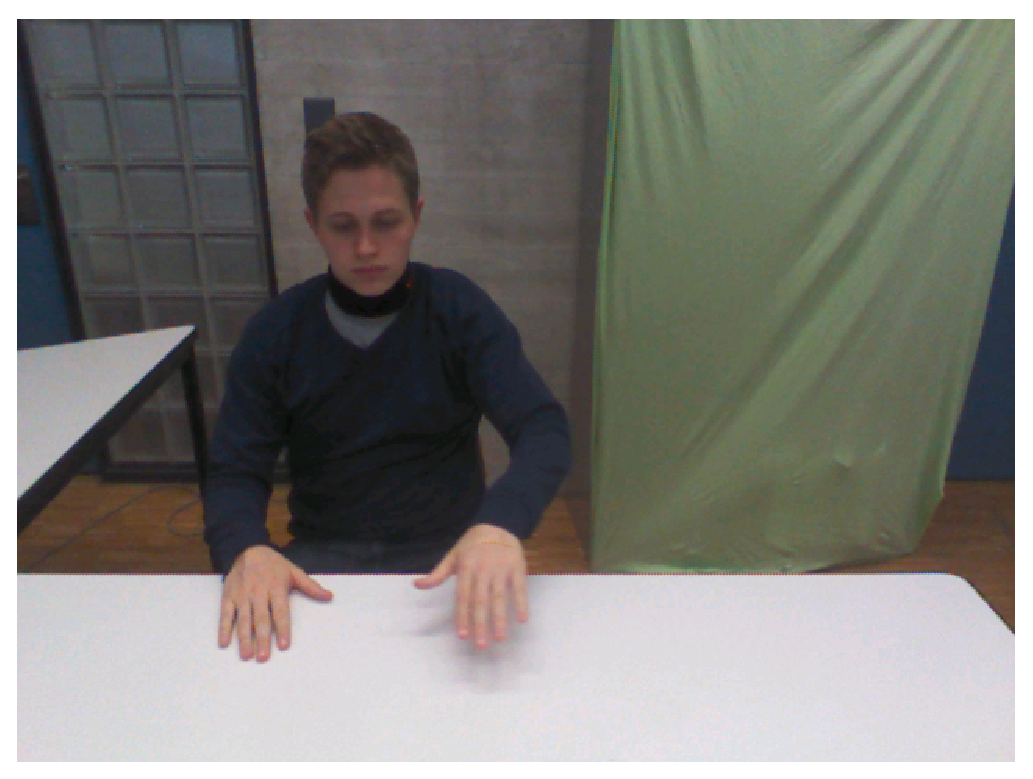
\includegraphics[width=0.24\linewidth]{figure/rotate-color.eps} \hspace{-0.6em}
}
\subfigure[]{
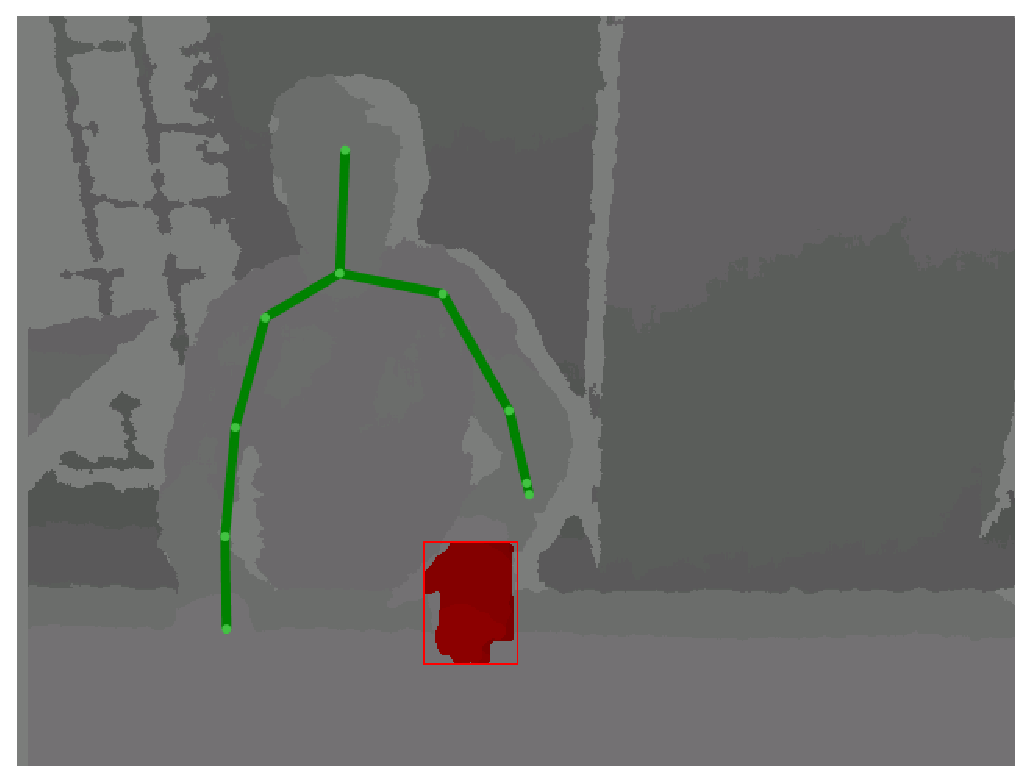
\includegraphics[width=0.24\linewidth]{figure/rotate-depth.eps} \hspace{-0.6em}
}
\subfigure[]{
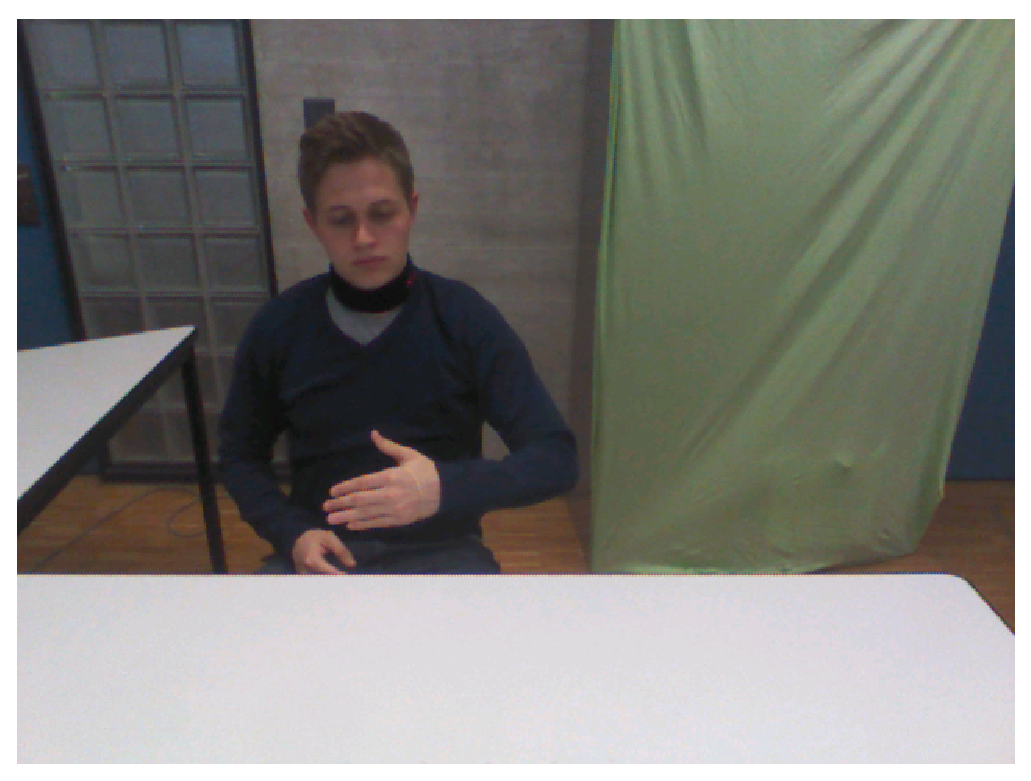
\includegraphics[width=0.24\linewidth]{figure/near-body-color.eps}
\hspace{-0.6em} }
\subfigure[]{
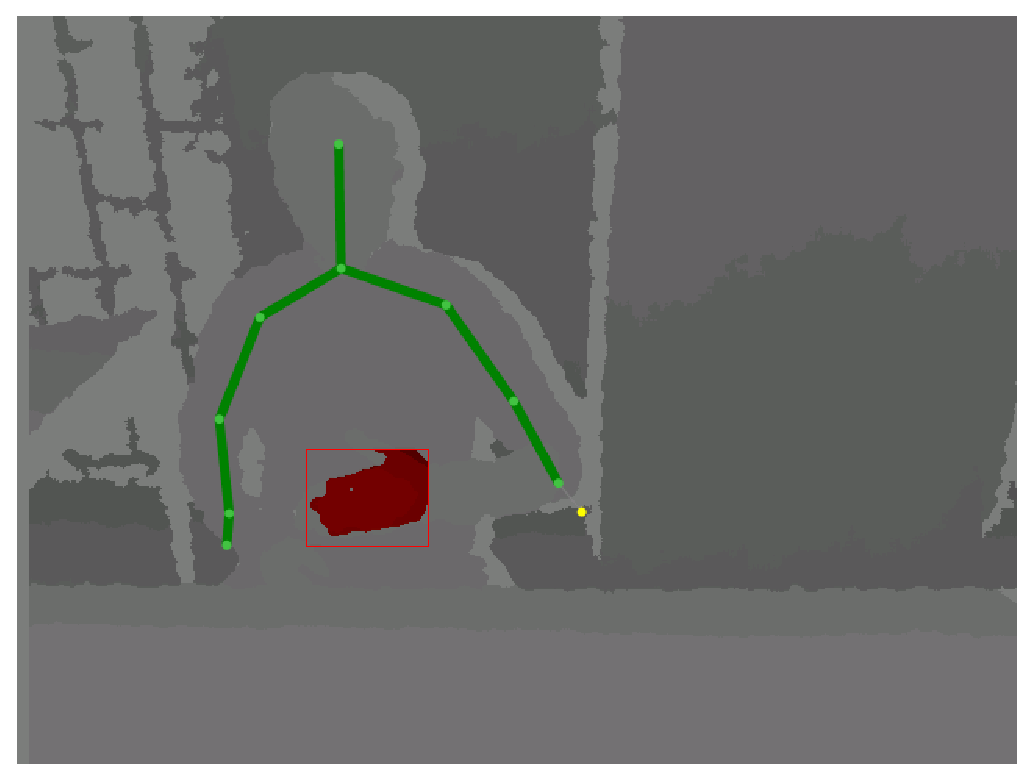
\includegraphics[width=0.24\linewidth]{figure/near-body-depth.eps}
\hspace{-0.6em} }
\caption{Comparison between gesture salience detection for hand gestures and skeleton tracking from the Kinect SDK. The green lines are
the skeleton tracking results. The red region is the detected salient gesture
region using our method. (Best viewed in color.)}
\label{fig:compare-skeleton}
\end{figure*}

\section{Online Continuous Gesture Recognition}
\subsection{Feature Descriptor}
From the bounding box, $B_t$, of the detected gesture salience, we compute both
a motion trajectory feature vector $X_t^M$ and a hand pose feature vector $X_t^P$. 

The motion trajectory feature vector $X_t^M$ includes relative
position from $B_t$ to the center of the shoulders
($\mathbf{p}$), velocity ($\mathbf{v}$), and acceleration ($\mathbf{a}$). The position of the shoulder center from the Kinect
skeleton tracking is consistently relatively accurate. The 3-dimensional
vectors $\mathbf{p}$, $\mathbf{v}$, $\mathbf{a}$ are in the world coordinate systems.

For hand pose features, we extract a depth-mapped $64\times 64$ px
image patch, $I_t$, from $B_t$.
We denoise, $I_t$, using a morphological close operation and then compute the
HOG feature descriptor~\cite{dalal05}, $I_t^H$, from it. The cell size we use is
$4\times 4$ px and the number of orientation bins is 9. Our earlier work (under
submission) shows that HOG descriptor with a small cell size for hand poses gives better
recognition accuracy. We also only use one fold of normalization because depth
values are less affected by illumination variation, and contrast normalization is
not necessary. The size of $I_t^H$ is thus $14\times 14\times 9$.

Similar to Wang et al.~\cite{wang-spatio-2009}, we apply dimension reduction on
$I_t^H$ using principal component analysis (PCA) on the
training data.
The final hand pose feature $X_t^P$ is obtained by projecting $I_t^H$ to a lower
dimensional space with dimension $k$.

The final feature vector $X_t$ combined from $X_t^M$ and $X_t^P$ has dimension
$9 + k$. Vectors are standardized to have zero mean and unit variance.
Figure~\ref{fig:feature} shows a visualization of the feature vectors (with $k=7$)
for a sequence of continuous gestures with rest poses in between. The regions of
smoothness indicate rest poses while the regions of rapid changes indicate
gestures.

\begin{figure}
\centering
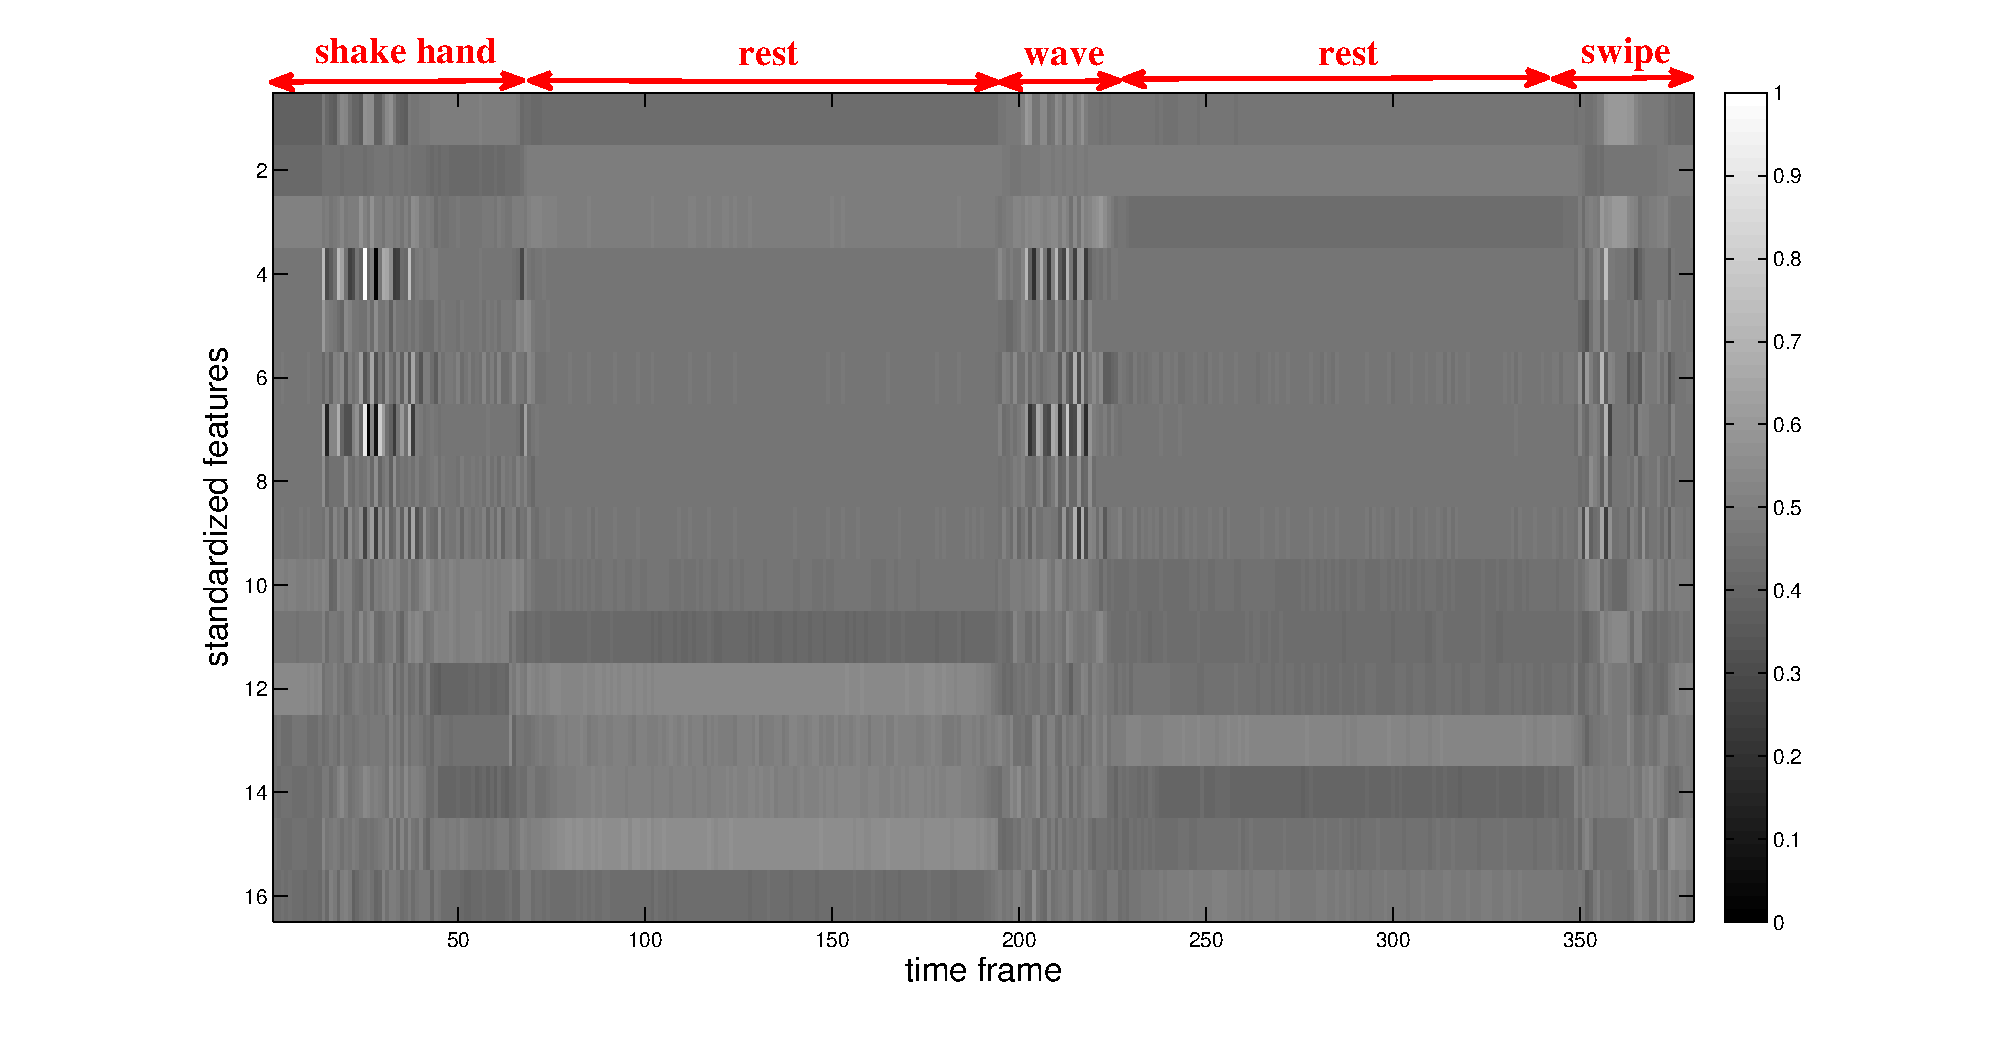
\includegraphics[width=1\columnwidth,trim=20mm 5mm 30mm 1mm,
clip]{figure/pca16.eps}
\caption{Visualization of a final feature vector sequence after dimension reduction and standardization.
The input is a gesture sequence with phases: ``shake hand'', ``rest'', ``wave'', ``rest'', and ``swipe''.}
\label{fig:feature}
\end{figure}

\subsection{Training AHMM for Gesture Recognition}
Our earlier work (under submission) has shown that the 1-level abstract hidden
Markov model (AHMM) closely models the gesture production process and
incorporates gesture recognition and gesture segmentation at the same time. 

Figure~\ref{fig:ahmm} shows the AHMM represented in a dynamic Bayesian network
(DBN). It is closely related to the hierarchical hidden Markov
model~\cite{murphy02}. Node $G_t$ represents the gesture that the
user is making at time $t$. It includes different gesture phases the system
can recognize.
Node $S_t$ is the hidden state of the hand movement, which is essentially a
vector quantization of the actual, observed (but noisy) feature vector $X_t$. 
Node $F_t^G$ is a binary variable that indicates the end of a
gesture. It is ``on'' (has value 1) if the lower level HMM at time $t$ has just
``finished'', otherwise it is ``off'' (value 0). $G_{t+1}$ can only change value
from $G_t$ if $F_t^G$ is ``on''. Note that $G_t$, $S_t$, and $F_t^G$ take
discrete values, hence their conditional probability distributions (CPDs)
can take a tabular form. $X_t$ is a vector with continuous values and we use a
Gaussian distribution for its CPD, i.e.,
\begin{align}
P(X_t = x_t | S_t = i) = N(x_t; \mu_i, \Sigma_i)
\end{align}

\begin{figure}
\centering
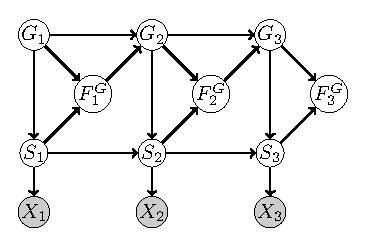
\includegraphics[]{figure/ahmm.eps}
\caption{One-level AHMM represented in DBN.}
\label{fig:ahmm}
\end{figure}

During the training process, we give the model sequences of difference gestures
with labeled $G_t$ and $F_t^G$ that correspond to the observed feature vectors
$X_t$, but $S_t$ is hidden. There can be different gestures in one sequence. In
this way, the model can learn the termination probability given a hidden state
and a gesture phase, i.e.,
$P(F_t^G = 1 | G_t = g, S_t = i)$, and the transition probability between two
hidden states given the gesture phase, i.e., $P(S_t = j | G_{t - 1} = g,
S_{t - 1} = i)$. Note that the transition probabilities learned are both
within and between gestures.

Compared with the mixture HMMs (Figure~\ref{fig:hmms}) previously used for gesture recognition,
AHMM allows sharing of substructures (i.e., hidden states $S_t$) across
different gestures and thus reduces the total number of hidden states. It is
also easier to learn the transition probabilities between hidden states across
gestures in AHMM than in the mixture of HMMs~\cite{murphy02}. In the experimental evaluation section, we give
a quantitative comparison between the two models for gesture recognition.

\tikzstyle{vertex}=[circle, draw, minimum size=16pt, inner sep=0pt]
\tikzstyle{observed-vertex}=[circle, draw, minimum size=16pt, inner
sep=0pt, fill=black!20] 
\tikzstyle{edge} = [draw, thick, -]
\tikzstyle{directed-edge} = [draw, thick, ->]

\begin{figure}[tb]
\centering
  \begin{tikzpicture}[auto,swap, scale=1.5]
    % First we draw the vertices
    \foreach \pos/\name in {{(1, 2)/G_1}, {(4,2)/G_2},
      {(0, 1)/S_{11}}, {(1, 1)/S_{12}}, {(2, 1)/S_{13}}, {(3, 1)/S_{21}}, {(4,
      1)/S_{22}}, {(5, 1)/S_{23}}} 
    \node[vertex] (\name) at \pos {$\name$};
    \foreach \pos/\name in {{(0, 0)/X_{11}}, {(1, 0)/X_{12}}, {(2, 0)/X_{13}},
    {(3, 0)/X_{21}}, {(4, 0)/X_{22}}, {(5, 0)/X_{23}}}
      \node[observed-vertex] (\name) at \pos {$\name$};
    % Connect vertices with edges and draw weights
    \foreach \source/ \dest in {G_1/S_{11}, G_1/S_{12}, G_1/S_{13},
    S_{11}/X_{11}, G_2/S_{21}, G_2/S_{22}, G_2/S_{23}, S_{12}/X_{12},
    S_{13}/X_{13}, S_{21}/X_{21}, S_{22}/X_{22}, S_{23}/X_{23}, S_{11}/S_{12}, S_{12}/S_{13},
    S_{21}/S_{22}, S_{22}/S_{23}} \path[directed-edge] (\source) -- (\dest);
  \end{tikzpicture}
  \caption{A mixture of HMMs~\cite{murphy02}.}
  \label{fig:hmms}
\end{figure}

Since $S_t$ is hidden, we use expectation maximization (EM)
algorithms to learn the maximum likelihood estimate of the model parameters for
all the CPDs. The performance of EM can be highly dependent on how the algorithm
is initialized~\cite{dicintio2012} and it tends to converge to a local maximum
of the observed data likelihood. As we model the $P(X_t | S_t)$ as a Gaussian
distribution, we can view $X_t$ as a mixture of Gaussians, and the number of hidden states 
$S_t$ can be the number of mixtures (i.e., clusters). Hence, we
perform an unsupervised clustering analysis on a sub-sample of the training data and
use the Bayesian information criterion (BIC)~\cite{fraley12} to find the optimal
number of clusters. We also initialize $\mu_i$ to be the cluster centers.

We compared the recognition accuracy using different clustering methods, including $k$-means,
and mixture of Gaussians with $k$-means initialization, multiple random
initializations, or hierarchical clustering initialization~\cite{Fraley:2003}. We
find that the hierarchical clustering initialization used in the \texttt{mclust} package in the R
language gives the best final recognition accuracy.

\subsection{Online Recognition}
Different inference methods exist for DBNs, including exact or approximate, offline or
online, with accuracy and speed trade-offs. As a first step, we use the
2TBN-based (2-slice temporal Bayes net) junction tree algorithm as the lower
level 
engine~\footnote{\url{http://bnt.googlecode.com/svn/trunk/docs/usage_dbn.html}}
to do exact inference on the graph. During the training process, we combine it
with the offline forwards-backwards message passing operators to smooth the
estimation using the entire evidence sequence.

During the online recognition process, we use the ``fixed-lag-smoothing''
method~\cite{murphy02} to allow a few frames lag in order to use more evidence to smooth the recognition result. This means, at time $t$,  we estimate the most likely
gesture at $t - L$ as:
\begin{align}
g* = \arg\max_g P(G_{t-L} = g | x_{1:t})
\end{align}
where $L$ is the lag time. At each time frame $t$, we compute the forward
message $\alpha_t(i)$ from $\alpha_{t-1}(i)$. Then we do a backward message passing
from $t$ to $t-L$ to smooth the gesture phase estimation at $t - L$.

\section{Experimental Evaluation}
Using a public gesture corpus
ChAirGest\cite{Ruffieux2013}, 
we conducted user-dependent evaluation to compare: 1)
feature detection methods; 2) feature descriptors; 3) gesture classification training
methods; and 4) online and offline inference.

\subsection{Data Set}
We use part of the ChAirGest corpus as our data set. We include data from
both lighting conditions: normal and low intensity. However we do not use the
data from the Xsens inertial measurement unit (IMU) sensors because we
think it is not likely that users would wear them in a realistic setting. We
only use the RGB, depth and skeleton stream data from the Kinect.

There are 10 gestures (swipe left (\#1), swipe right (\#2), push to screen
(\#3), take from screen (\#4), palm-up rotation (\#5), palm-down rotation (\#6),
draw a circle with rotating palm (\#7), draw a circle with palm down (\#8), wave
hello (\#9) and shake hand (\#10)) and 3 resting postures (hands on then table,
hands on the belly , and hands under the chin) in the corpus.
Each gesture consists of labeled pre-stroke, gesture nucleus and
post-stroke~\cite{Pavlovic97} phases.

We use recordings from 8 participants,and for each participant, we use 2 sessions
of recordings\footnote{Data from 2 out of the 10 participants are corrupted.}.
In each session, there are 7-8 sequences with 2-5 gesture occurrences per
sequence. Overall there are 2 occurrence for each gesture/resting posture combination per subject.

\subsection{Method}
For each participant, we use
one tenth of the sequences for testing and the remaining for training. 
The RGB and depth videos are 30 fps (frame per second) and we down-sample them
to 10 fps to increase the training speed. This results in about 600 frames per sequence on average.

We treat the preparation phase (\#11), the retraction phase (\#12) and the rest posture (\#13) 
as different gesture classes, resulting
in 13 gesture classes. The a random guess accuracy would be
7.8\%.


In this data set, all gesture occurrences follow the pattern: rest $\rightarrow$ preparation
$\rightarrow$ gesture nucleus $\rightarrow$ retraction $\rightarrow$ rest and then repeat. 
Hence, we initialize the prior distribution CPD
and the transition probability CPD for $G_t$ such that the probability of transition from the preparation phase
to one of the ten gesture nucleus phases is uniform and all other transitions are deterministic.

We use features computed using our method described in the earlier section based
on the training data from one participant to do mixture of Gaussian clustering analysis\footnote{\url{http://cran.r-project.org/web/packages/mclust/index.html}}. 
Our results show that $50$ clusters and
$11$ features give the highest BIC. Hence we set the 
number of hidden states $S_t$ to be $50$ and $k = 2$
during PCA dimensionality reduction of the hand pose feature $X_t^P$.

To compare recognition performance, we compute per frame accuracy and F1 score. 
A frame is considered correctly classified if its predicted label is equal to the ground truth label.
Hence frame accuracy is computed as
\begin{displaymath}
\text{frame accuracy} = \frac{\text{\# correctly classified frames}}{\text{\# frames in the sequence}}
\end{displaymath}
Because we have a multi-class classification problem, we compute an F1 score for each gesture class, with an 
 overall F1 score computed as the average from all gesture classes. All results
reported here are for the test data set.

\subsection{Comparison of Feature Detection Methods}
% \begin{table}
%   \centering
%   \begin{tabular}{|c|c|c|}
%     \hline
%     \tabhead{Objects} &
%     \multicolumn{1}{|p{0.3\columnwidth}|}{\centering\tabhead{Caption --- pre-2002}} &
%     \multicolumn{1}{|p{0.4\columnwidth}|}{\centering\tabhead{Caption --- 2003 and afterwards}} \\
%     \hline
%     Tables & Above & Below \\
%     \hline
%     Figures & Below & Below \\
%     \hline
%   \end{tabular}
%   \caption{Table captions should be placed below the table.}
%   \label{tab:table1}
% \end{table}
We compare our gesture salience feature detection method with two other
methods based on their effect on gesture recognition performance (see Table~\ref{tab:feature-detection}). 

As mentioned in Related Work, Dense sampling is the simplest method which extracts features at
regular positions in a image. Skin \& Kinect skeleton method finds the skin contour closest to the right hand
joint from the skeleton tracking provided by Microsoft's Kinect SDK.

We use the same HOG feature descriptor with $4\times 4$ px cell size and 9
orientation bins, and reduce the feature dimension using PCA.
No motion trajectory features are used for dense sampling, while the
9-dimensional motion trajectory feature $X^M$ is included for both Skin \&
Kinect skeleton method and gesture salience method.
Table~\ref{tab:feature-detection} shows their performance on gesture recognition using the same AHMM-based recognition method with offline smoothing.

\begin{table}
\centering
\begin{tabular}{|l|l|l|}
\hline
\tabhead{Feature detector} & {\tabhead{Accuracy (std.)}} & {\tabhead{F1 (std.)}}\\
\hline
Dense sampling upper body & 68.0\% (4) & 57.7\% (8)\\
\hline
Skin \& Kinect skeleton & 72.1\% (16) & 64.7\% (11) \\
\hline
Gesture salience & \textbf{76.7\%} (4) & \textbf{69.3\%} (6) \\
\hline
\end{tabular}
\caption{Comparison of different feature detection methods.}
\label{tab:feature-detection}
\end{table}

The results show that our salience detection method gives the best performance.
It is possible that dense sampling may work better for gestures with big arm
movements away from the body, but our data set contains gestures with
small movement, close to the body (e.g., swipe left/right, take from screen).

The lower performance using skin \& Kinect skeleton method shows that error
in feature location detection (in this case due to error in skin detection and
skeleton tracking) will affect the recognition performance.

\subsection{Comparison of Feature Descriptor}
We also compare the recognition results without and with the hand pose feature
$X_t^P$. The results in Table~\ref{tab:hand-pose-feature} shows that the
performance is comparable, with the results using the hand pose feature very
slightly higher. This may be due to the fact that most of the gestures in the
data set are distinguishable based on motion trajectory and hand pose may play a relatively minor role. However, by comparing
Figure~\ref{fig:cm9} and \ref{fig:cm11}, we can see that the hand pose features
still help improve the recognition accuracy for certain gestures such as ``swipe right'' (\#2), ``push to screen'' (\#3), ``take from screen'' (\#4).
The ``take from screen'' has a dynamic hand pose (grab motion) and hence, the hand
pose feature can provide additional information for its recognition.

We also note that the noise in hand pose features due to variations in the
locations of the center of salience can also contribute to the decrease in
recognition accuracy for some gestures.

\begin{table}
\centering
\begin{tabular}{|l|l|l|}
\hline
\tabhead{Hand pose feature} & \tabhead{Accuracy (std.)} & \tabhead{F1 (std.)}\\
\hline
No hand pose feature & 76.5\% (5) & 68.4\% (7)\\
\hline
Use hand pose feature  & \textbf{76.7\%} (4) & \textbf{69.3\%} (6) \\
\hline
\end{tabular}
\caption{Comparison of excluding hand pose features vs. including hand pose features in gesture recognition.}
\label{tab:hand-pose-feature}
\end{table}

\begin{figure}
\centering
\hspace{-8.5755mm}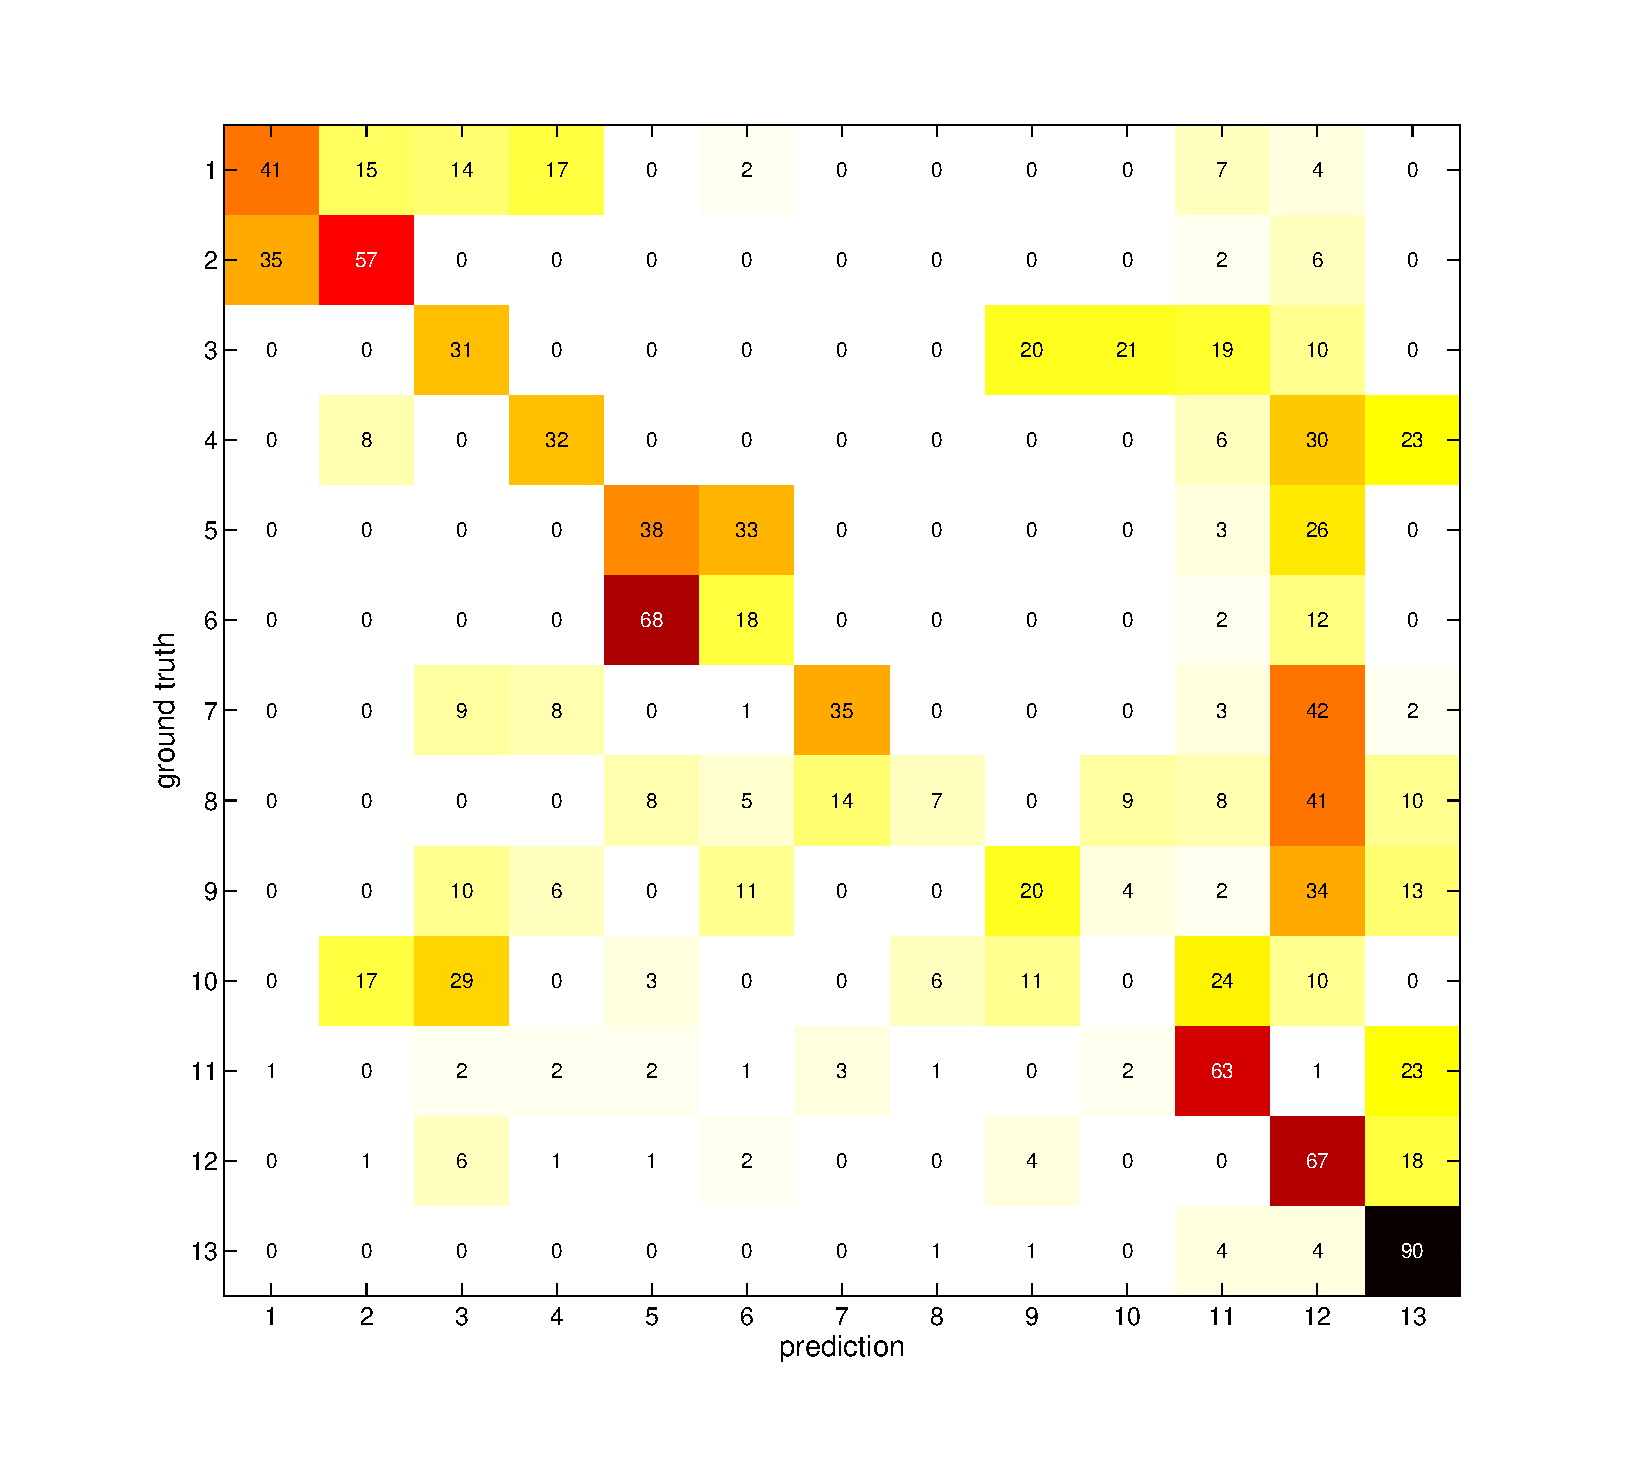
\includegraphics[width=1.05\columnwidth]{figure/cm9.eps}
\caption{Confusion matrix of ground truth gesture phase labels vs. predicted
gesture phase labels per frame when \textit{no hand pose features} are used. Darker
color indicates higher accuracy.}
\label{fig:cm9}
\end{figure}

\begin{figure}
\centering
\hspace{-8.5755mm}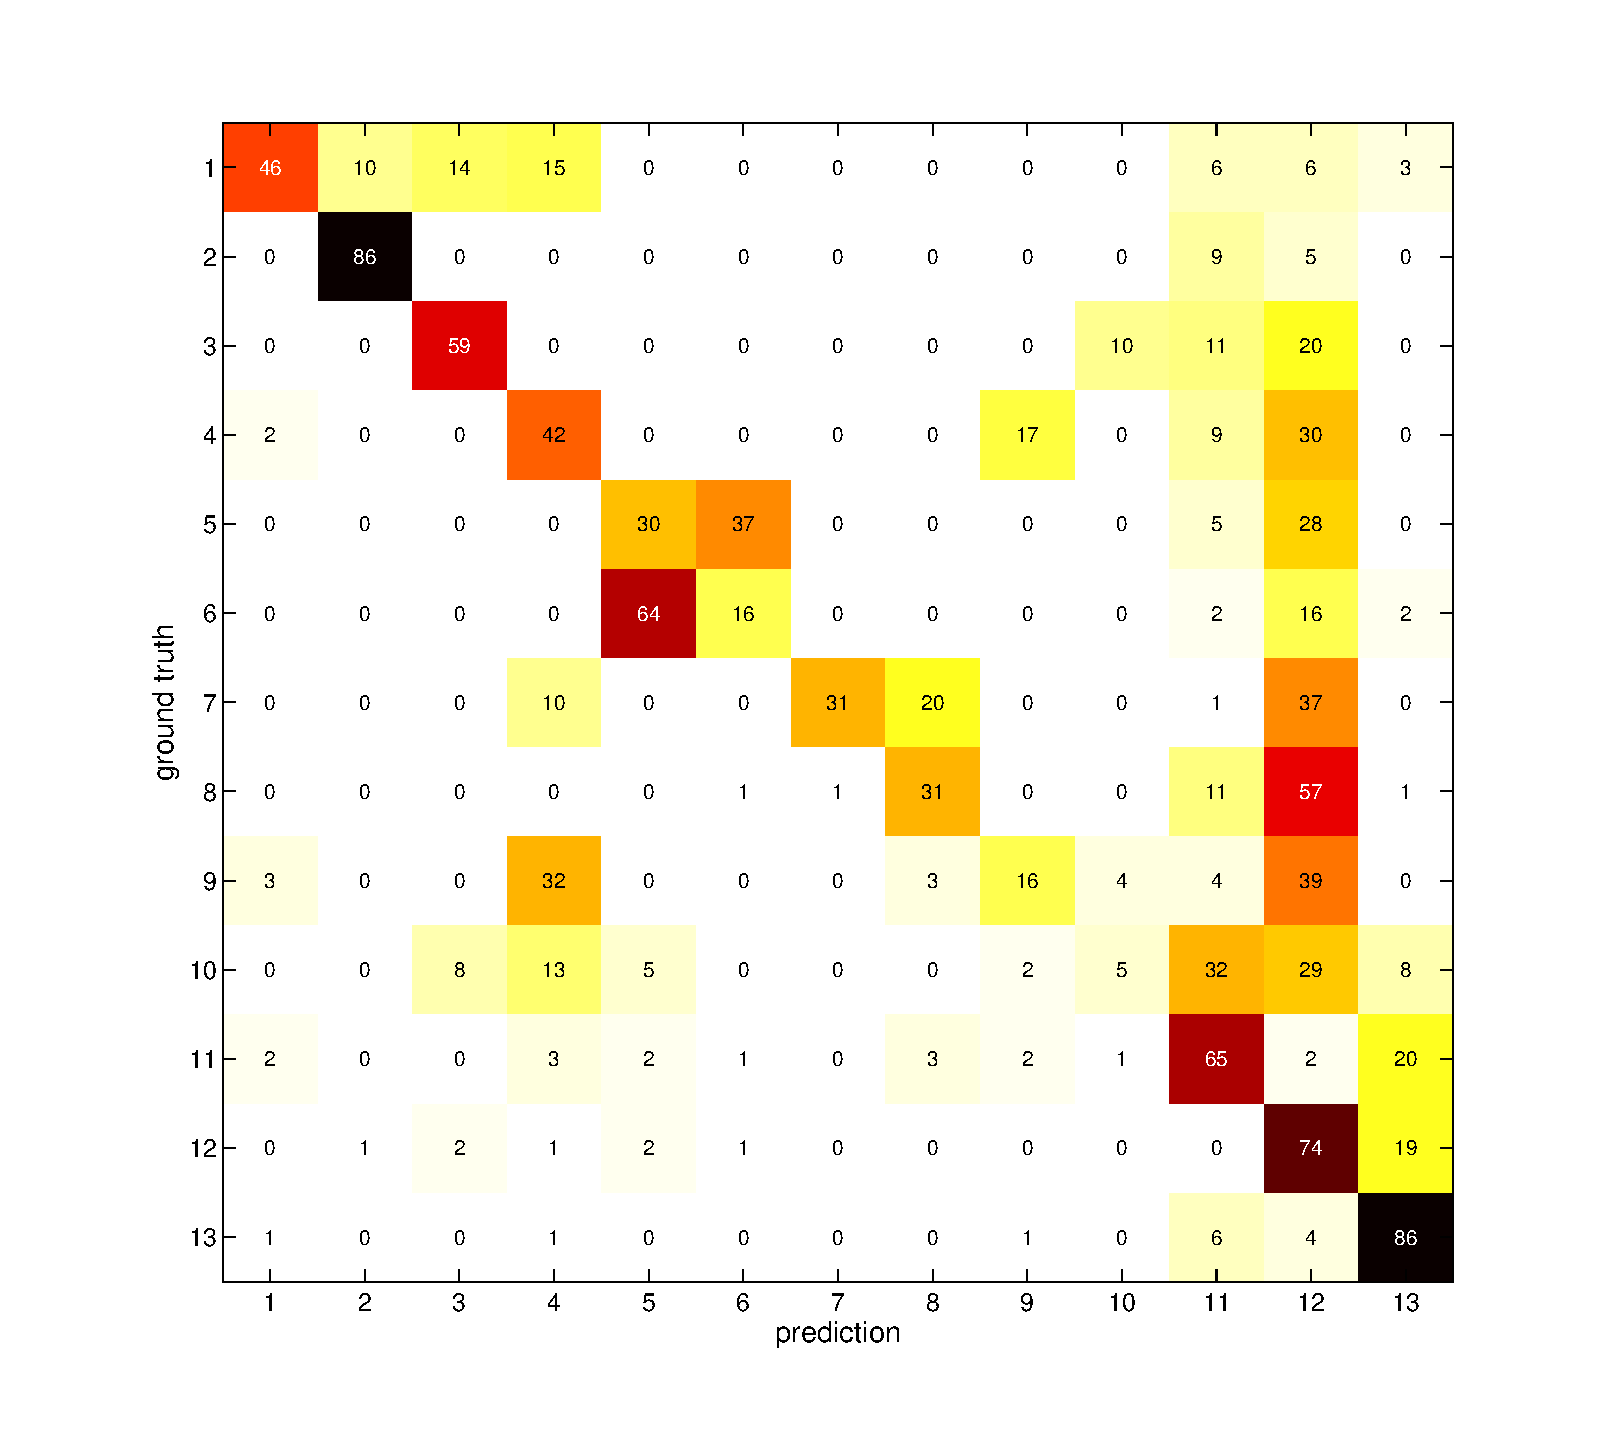
\includegraphics[width=1.05\columnwidth]{figure/cm11.eps}
\caption{Confusion matrix of ground truth gesture phase labels vs. predicted
gesture phase labels per frame when \textit{hand pose features} are used
($k=2$). Darker
color indicates higher accuracy.}
\label{fig:cm11}
\end{figure}

\subsection{Comparison of Classification Training Methods}
We gave a qualitative comparison between the AHMM and the mixture HMMs for
gesture recognition in the earlier section. Here we report our experimental
evaluation using two models to train the parameters. The best salience feature detector and descriptor
described from the earlier sections are used for both training methods. Offline
smoothing is used for recognition in both cases. 

To train the mixture of HMMs, we segment the training sequences for each gesture
phase. For each gesture HMM, we use 5 hidden states and initialize the
transition probabilities uniformly. The means of the Gaussian distribution CPD
$P(X_t|S_gt)$ are initialized using mixture of Gaussians clustering as well. We
also learn the termination probability of each hidden state for gesture phase
$g$.

As the mixture of HMMs do not handle termination and transition directly, for gesture classification we apply
the learned parameters to a hierarchical HMM shown in
Figure~\ref{fig:ahmm-reset}. This model is similar to AHMM in
Figure~\ref{fig:ahmm} with one distinction: the hidden state $S_t$ resets if
the previous gesture terminates (represented by the directed edge from $F_t^G$
to $S_t$). In this case, the prior probability, i.e., $P(S_1 = j | G_1 = i)$
learned in the mixture of HMMs can be used.

\begin{figure}
\centering
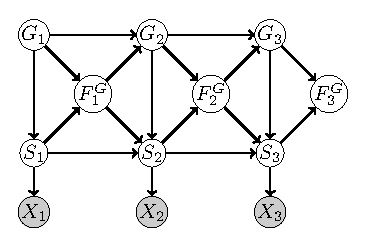
\includegraphics[]{figure/ahmm-reset.eps}
\caption{Hierarchical HMM with hidden state $S_t$ reset when the previous gesture terminates.}
\label{fig:ahmm-reset}
\end{figure}

The advantage of HMM training is that it reduces the total number of
state transition parameters to be learned and hence reduces the
complexity of the model. The inference algorithm on HMM can be faster than
the junction tree algorithm. However, the results in Table~\ref{tab:training}
show that the performance using a mixture of HMMs training is much lower, showing
that the state transition probabilities across the gestures can help improve the
gesture recognition accuracy.

\begin{table}[t]
\centering
\begin{tabular}{|l|l|l|}
\hline
\tabhead{Training method} & {\tabhead{Accuracy (std.)}} & {\tabhead{F1 (std).}}\\
\hline
Mixture of HMMs & 50.6\% (17) & 55.6\% (8) \\
\hline
AHMM & \textbf{76.7\%} (4) & \textbf{69.3\%} (6) \\
\hline
\end{tabular}
\caption{Comparison of gesture recognition performance from models trained from a mixture of HMMs and an AHMM.}
\label{tab:training}
\end{table}

\subsection{Comparison of Online and Offline Inference}
Table~\ref{tab:inference} shows that our online inference method with a 16-frame lag gives results comparable to offline inference. This is a promising result because with 30fps data
stream, 16 frames is about half a second delay, which might acceptable for human
reaction time.

\begin{table}[t]
\centering
\begin{tabular}{|l|l|l|}
\hline
\tabhead{Inference} & {\tabhead{Accuracy (std.)}} & {\tabhead{F1 (std).}}\\
\hline
Offline & 76.7\% (4) & 69.3\% (6) \\
\hline
Online (lag = 16 frames) & \textbf{76.9\%} (3) & \textbf{65.2\%} (9) \\ 
\hline
\end{tabular}
\caption{Comparison of gesture recognition performance between offline and online inference. }
\label{tab:inference}
\end{table}


\section{Future Work}
Our gesture salience detection method gives better recognition performance than the dense sampling method and
the one using the Kinect skeleton tracking. However as our method still relies on skin color detection to filter
the noise from the depth camera, there still can be failure modes when the users wear gloves or hold something
in their hands. In fact, this happens in the data set we use. The IMU attached to the user's hand affects the 
skin color detection and makes holes in the hand image. This could cause the noise in the hand pose features. In the future,
we would like to avoid using skin color detection. 

Currently, when the user is not moving, we still compute the image feature at the gesture salience region from the previous time frame.
Wrong detection occurs when the user is not moving his/her hand, but the system still detects motion due to noise near the hair region.
We will consider using an empty image when there is no motion and compare the recognition performance.

\section{Conclusion}
We have developed a gesture salience detection method for gesture recognition. It shows a better result than both dense sampling and using 
Kinect skeleton tracking.

Our AHMM based recognition framework allows for online continuous gesture recognition. A small time lag (~0.5s) can give comparable results with offline
smoothing.

Our evaluation also show that AHMM based recognition gives better results than the mixture of HMMs method because it learns transition probabilities across gestures,
 and sharing of hidden states allows more examples be pooled together for training.

% It is important that you write for the SIGCHI audience.  Please read
% previous years' Proceedings to understand the writing style and
% conventions that successful authors have used.  It is particularly
% important that you state clearly what you have done, not merely what
% you plan to do, and explain how your work is different from previously
% published work, i.e., what is the unique contribution that your work
% makes to the field?  Please consider what the reader will learn from
% your submission, and how they will find your work useful.  If you
% write with these questions in mind, your work is more likely to be
% successful, both in being accepted into the Conference, and in
% influencing the work of our field.

% Balancing columns in a ref list is a bit of a pain because you
% either use a hack like flushend or balance, or manually insert
% a column break.  http://www.tex.ac.uk/cgi-bin/texfaq2html?label=balance
% multicols doesn't work because we're already in two-column mode,
% and flushend isn't awesome, so I choose balance.  See this
% for more info: http://cs.brown.edu/system/software/latex/doc/balance.pdf
%
% Note that in a perfect world balance wants to be in the first
% column of the last page.
%
% If balance doesn't work for you, you can remove that and
% hard-code a column break into the bbl file right before you
% submit:
%
% http://stackoverflow.com/questions/2149854/how-to-manually-equalize-columns-
% in-an-ieee-paper-if-using-bibtex
%
% Or, just remove \balance and give up on balancing the last page.
%
\balance

% If you want to use smaller typesetting for the reference list,
% uncomment the following line:
% \small
\bibliographystyle{acm-sigchi}
\bibliography{gesture}
\end{document}
